%!TEX root = ../thesis.tex

\cleardoublepage
\chapter{Approach}
\label{cha:approach}


This chapter covers how the problem was addressed and how the proposed solution was integrated into a scientific workflow manager and tested. This chapter will first look over the software architecture of the approach and where it was inserted into the source code of nextflow, then the exact nature of the gradient bandit and the q-learning approaches will be considered. After that some initial issues which were encountered and the solutions to them will be mentioned and then finally the nature of the tests will briefly be introduced before the results from those tests are presented in the following chapter. 

%%=========================================
\section{Integrating a Solution in a Workflow Manager}
\label{sec:integration}

Nextflow is a very robust scientific  workflow management system written primarily in groovy. It supports various execution platforms and has a large variety of tools to help users analyse the performance of their workflows \cite{TracingAndVisualisation}. Nextflow is free open source software and for this thesis a fork of the 20.12.0 version was used. In order to integrate a reinforcement learning approach with the nextflow source code a simple structure was designed which externalised the storage of the data of previous tasks and workflow runs to a database and when a task needed to be scheduled, the reinforcement learning agent would use the historical data for that task to inform its decision. The structure can be seen in the following figure.

\begin{figure}[ht]
    \centering
        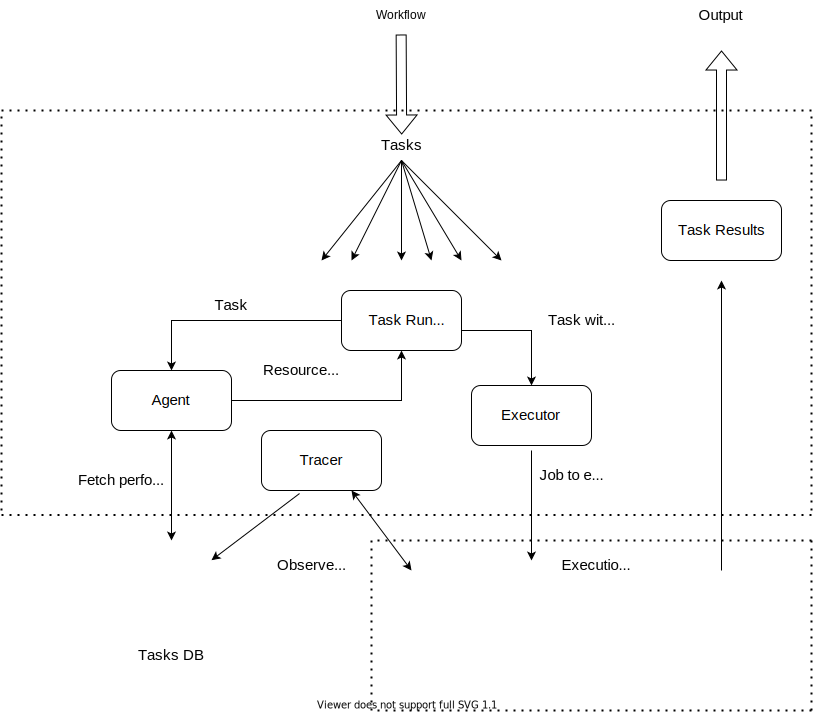
\includegraphics[width=0.8\textwidth]{fig/implementation_diagram.png}
        \caption{High Level Design: Integration of a Reinforcement-Learning Agent with Nextflow}
        \label{fig:implementation}
\end{figure}

Before a task is ready to be scheduled it is first sent to the reinforcement-learning agent specific to that task. For the purposes of this thesis that was either a q-learning agent or a gradient bandit. The task’s agent would then select historical performance data and any other relevant data (i.e. what state the agent was last in) from the database. This database is external to nextflow and the creation and management of this database is not performed by nextflow or the agent- nextflow and the agent only use the database to store or read data. Using this data, the agent selects a new resource allocation for the task and overwrites the task’s default configuration. After this nextflow uses its custom executor for the given execution platform to prepare the task and pass it on to that platform. The task is then executed. It is important to note that the execution platform will also have its own system for managing, scheduling and executing jobs and processes but from the perspective of the nextflow/agent system all it does is pass on the task with the resource allocations which were chosen. As the task is executed nextflow’s tracer module will \cite{TracingAndVisualisation} gather performance data, i.e. peak CPU usage, peak RSS and other such things. Once the task is finished all of this data is stored in the  database to be used by the agent the next time the task comes. It is important to note that there is one agent for each unique task. These agents are called up whenever their task needs to be executed and they all use the database to receive feedback about their performance.

\section{Reinforcement Learning Approaches}
\label{sec:rl_approaches}

Now that the structure of the agent’s environment has been explained and the relationship between task scheduling and collecting data about a task is clear, it is time to delve into the specific approaches tried. In total there were 2 different approaches considered. There was a gradient bandit which only chose how many cpu’s to assign and a q-learning agent which had as its state the current allocation of cpu and memory for the given task, and as its set of actions it could choose between incrementing or decrementing the amount of cpus or memory, or it could do nothing.

\subsection{CPU Bandit}
\label{sub:cpu_bandit}

The first bandit or CPU Bandit, as it was nicknamed, was based on a very straightforward reward function:

\begin{equation}\label{bandit1_reward}
reward = -t*(1+cpus - cpu\_usage/100)
\end{equation}


In this equation $cpu\_usage$ is a value in percent of the number of single core CPUs used by the task. If a task where assigned 4 CPUs and only ever used two of them then $cpu\_usage$ would be $200$\%. $cpus$ is of course the number of CPUs assigned to the task and $t$ stands for time- it is a measure of how long the task ran. Put in other words this equation punishes the agent with a negative reward equal to the amount of time it ran plus the amount of unused CPU time. The idea is that the agent is incentivised to try to minimise the amount of time where any of the allocated CPU’s are not being used, but by also punishing it with the amount of time that the task ran for the agent is also encouraged to try to reduce the amount of time taken for the task to complete. Additionally, should a task have 100\% usage then its penalty is not 0 but is just the time that it ran. The reason for this is that if the agent has no concept of time it will always allocate the least amount of resources possible since that immediately minimises the amount of resources wasted, and ultimately the tasks and their workflows would be incredibly slow. 

It should be noted here that the image of the function $r(cpus,cpu\_usage,time)$ where $r$ is the equation from \ref{bandit1_reward} is bounded by [ $-time$ , $time*(cpus+1)$ ]. This will become relevant in \ref{sec:initial_problems}. The bandit’s other parameter- the step size $\alpha$ was initially set to $0.1$. 

\subsection{Q-Agent}
\label{sub:q_agent}

For the Q-Agent a different reward function was used, primarily because it also had to incorporate memory but also as part of an attempt to try slightly different reward functions. 

\begin{equation}\label{q_agent_1_reward}
r = -max(0.1,cpus-cpu\_usage/100) * (t/avg\_t) * (mem* (1 - max(0.75,mem\_usage/100)))
\end{equation}

Here the $memory$ variable refers to the memory allocated to the process and $mem\_usage$ is the value of of the peak RSS of the process divided by the memory assigned to it. $avg\_t$ is a constant value which is determined at runtime based on the historical average execution time for the task. This function is effectively a product of the number of unused CPUs, the slow-down factor and the amount of unused memory. There are some slight modifications though. The $max$ function is used to set an artificial floor for the penalty incurred by the unused CPUs and unused memory. Tasks which use more than 90\% of the available CPUs are given the same reward as tasks which use exactly 90\% in an attempt to prevent the agent from deciding to assign each task 1 CPU in order to minimise the amount of unused CPUs. Additionally the floor for unused memory is capped at 25\% in a similar manner. This is done to discourage the agent from allocating too little memory because tasks which use too much memory will of course be killed and have to start over, which has a hugely detrimental effect on performance. This reward function is of course negated in order to turn it into a penalty function so that the agent will seek to minimise its penalty by minimising the unused CPUs, slowdown and unused memory.

\section{Initial Problems}
\label{sec:initial_problems}

\section{Testing the Agents}
\label{sec:testing}